
\documentclass[letterpaper,hide notes,xcolor={table,svgnames},pdftex,10pt]{beamer}
\def\showexamples{t}


%\usepackage[svgnames]{xcolor}

%% Demo talk
%\documentclass[letterpaper,notes=show]{beamer}

\usecolortheme{crane}
\setbeamertemplate{navigation symbols}{}

\usetheme{MyPittsburgh}
%\usetheme{Frankfurt}

%\usepackage{tipa}

\usepackage{hyperref}
\usepackage{graphicx,xspace}
\usepackage[normalem]{ulem}
\usepackage{multicol}

\newcommand\SF[1]{$\bigstar$\footnote{SF: #1}}

\usepackage[default]{sourcesanspro}
\usepackage[T1]{fontenc}

\newcounter{tmpnumSlide}
\newcounter{tmpnumNote}

% old question code
%\newcommand\question[1]{{$\bigstar$ \small \onlySlide{2}{#1}}}
% \newcommand\nquestion[1]{\ifdefined \presentationonly \textcircled{?} \fi \note{\par{\Large \textbf{?}} #1}}
% \newcommand\nanswer[1]{\note{\par{\Large \textbf{A}} #1}}


 \newcommand\mnote[1]{%
   \addtocounter{tmpnumSlide}{1}
   \ifdefined\showcues {~\tiny\fbox{\arabic{tmpnumSlide}}}\fi
   \note{\setlength{\parskip}{1ex}\addtocounter{tmpnumNote}{1}\textbf{\Large \arabic{tmpnumNote}:} {#1\par}}}

\newcommand\mmnote[1]{\note{\setlength{\parskip}{1ex}#1\par}}

%\newcommand\mnote[2][]{\ifdefined\handoutwithnotes {~\tiny\fbox{#1}}\fi
% \note{\setlength{\parskip}{1ex}\textbf{\Large #1:} #2\par}}

%\newcommand\mnote[2][]{{\tiny\fbox{#1}} \note{\setlength{\parskip}{1ex}\textbf{\Large #1:} #2\par}}

\newcommand\mquestion[2]{{~\color{red}\fbox{?}}\note{\setlength{\parskip}{1ex}\par{\Large \textbf{?}} #1} \note{\setlength{\parskip}{1ex}\par{\Large \textbf{A}} #2\par}\ifdefined \presentationonly \pause \fi}

\newcommand\blackboard[1]{%
\ifdefined   \showblackboard
  {#1}
  \else {\begin{center} \fbox{\colorbox{blue!30}{%
         \begin{minipage}{.95\linewidth}%
           \hspace{\stretch{1}} Some space intentionally left blank; done at the blackboard.%
         \end{minipage}}}\end{center}}%
         \fi%
}



%\newcommand\q{\tikz \node[thick,color=black,shape=circle]{?};}
%\newcommand\q{\ifdefined \presentationonly \textcircled{?} \fi}

\usepackage{listings}
\lstset{%
  keywordstyle=\bfseries,
  aboveskip=15pt,
  belowskip=15pt,
  captionpos=b,
  identifierstyle=\ttfamily,
  escapeinside={(*@}{@*)},
  stringstyle=\ttfamiliy,
  frame=lines,
  numbers=left, basicstyle=\scriptsize, numberstyle=\tiny, stepnumber=0, numbersep=2pt}

\usepackage{siunitx}
\newcommand\sius[1]{\num[group-separator = {,}]{#1}\si{\micro\second}}
\newcommand\sims[1]{\num[group-separator = {,}]{#1}\si{\milli\second}}
\newcommand\sins[1]{\num[group-separator = {,}]{#1}\si{\nano\second}}
\sisetup{group-separator = {,}, group-digits = true}

%% -------------------- tikz --------------------
\usepackage{tikz}
\usetikzlibrary{positioning}
\usetikzlibrary{arrows,backgrounds,automata,decorations.shapes,decorations.pathmorphing,decorations.markings,decorations.text}

\tikzstyle{place}=[circle,draw=blue!50,fill=blue!20,thick, inner sep=0pt,minimum size=6mm]
\tikzstyle{transition}=[rectangle,draw=black!50,fill=black!20,thick, inner sep=0pt,minimum size=4mm]

\tikzstyle{block}=[rectangle,draw=black, thick, inner sep=5pt]
\tikzstyle{bullet}=[circle,draw=black, fill=black, thin, inner sep=2pt]

\tikzstyle{pre}=[<-,shorten <=1pt,>=stealth',semithick]
\tikzstyle{post}=[->,shorten >=1pt,>=stealth',semithick]
\tikzstyle{bi}=[<->,shorten >=1pt,shorten <=1pt, >=stealth',semithick]

\tikzstyle{mut}=[-,>=stealth',semithick]

\tikzstyle{treereset}=[dashed,->, shorten >=1pt,>=stealth',thin]

\usepackage{ifmtarg}
\usepackage{xifthen}
\makeatletter
% new counter to now which frame it is within the sequence
\newcounter{multiframecounter}
% initialize buffer for previously used frame title
\gdef\lastframetitle{\textit{undefined}}
% new environment for a multi-frame
\newenvironment{multiframe}[1][]{%
\ifthenelse{\isempty{#1}}{%
% if no frame title was set via optional parameter,
% only increase sequence counter by 1
\addtocounter{multiframecounter}{1}%
}{%
% new frame title has been provided, thus
% reset sequence counter to 1 and buffer frame title for later use
\setcounter{multiframecounter}{1}%
\gdef\lastframetitle{#1}%
}%
% start conventional frame environment and
% automatically set frame title followed by sequence counter
\begin{frame}%
\frametitle{\lastframetitle~{\normalfont(\arabic{multiframecounter})}}%
}{%
\end{frame}%
}
\makeatother

\makeatletter
\newdimen\tu@tmpa%
\newdimen\ydiffl%
\newdimen\xdiffl%
\newcommand\ydiff[2]{%
    \coordinate (tmpnamea) at (#1);%
    \coordinate (tmpnameb) at (#2);%
    \pgfextracty{\tu@tmpa}{\pgfpointanchor{tmpnamea}{center}}%
    \pgfextracty{\ydiffl}{\pgfpointanchor{tmpnameb}{center}}%
    \advance\ydiffl by -\tu@tmpa%
}
\newcommand\xdiff[2]{%
    \coordinate (tmpnamea) at (#1);%
    \coordinate (tmpnameb) at (#2);%
    \pgfextractx{\tu@tmpa}{\pgfpointanchor{tmpnamea}{center}}%
    \pgfextractx{\xdiffl}{\pgfpointanchor{tmpnameb}{center}}%
    \advance\xdiffl by -\tu@tmpa%
}
\makeatother
\newcommand{\copyrightbox}[3][r]{%
\begin{tikzpicture}%
\node[inner sep=0pt,minimum size=2em](ciimage){#2};
\usefont{OT1}{phv}{n}{n}\fontsize{4}{4}\selectfont
\ydiff{ciimage.south}{ciimage.north}
\xdiff{ciimage.west}{ciimage.east}
\ifthenelse{\equal{#1}{r}}{%
\node[inner sep=0pt,right=1ex of ciimage.south east,anchor=north west,rotate=90]%
{\raggedleft\color{black!50}\parbox{\the\ydiffl}{\raggedright{}#3}};%
}{%
\ifthenelse{\equal{#1}{l}}{%
\node[inner sep=0pt,right=1ex of ciimage.south west,anchor=south west,rotate=90]%
{\raggedleft\color{black!50}\parbox{\the\ydiffl}{\raggedright{}#3}};%
}{%
\node[inner sep=0pt,below=1ex of ciimage.south west,anchor=north west]%
{\raggedleft\color{black!50}\parbox{\the\xdiffl}{\raggedright{}#3}};%
}
}
\end{tikzpicture}
}


%% --------------------

%\usepackage[excludeor]{everyhook}
%\PushPreHook{par}{\setbox0=\lastbox\llap{MUH}}\box0}

%\vspace*{\stretch{1}

%\setbox0=\lastbox \llap{\textbullet\enskip}\box0}

\setlength{\parskip}{\fill}

\newcommand\noskips{\setlength{\parskip}{1ex}}
\newcommand\doskips{\setlength{\parskip}{\fill}}

\newcommand\xx{\par\vspace*{\stretch{1}}\par}
\newcommand\xxs{\par\vspace*{2ex}\par}
\newcommand\tuple[1]{\langle #1 \rangle}
\newcommand\code[1]{{\sf \footnotesize #1}}
\newcommand\ex[1]{\uline{Example:} \ifdefined \presentationonly \pause \fi
  \ifdefined\showexamples#1\xspace\else{\uline{\hspace*{2cm}}}\fi}

\newcommand\ceil[1]{\lceil #1 \rceil}


\AtBeginSection[]
{
   \begin{frame}
       \frametitle{Outline}
       \tableofcontents[currentsection]
   \end{frame}
}



\pgfdeclarelayer{edgelayer}
\pgfdeclarelayer{nodelayer}
\pgfsetlayers{edgelayer,nodelayer,main}

\tikzstyle{none}=[inner sep=0pt]
\tikzstyle{rn}=[circle,fill=Red,draw=Black,line width=0.8 pt]
\tikzstyle{gn}=[circle,fill=Lime,draw=Black,line width=0.8 pt]
\tikzstyle{yn}=[circle,fill=Yellow,draw=Black,line width=0.8 pt]
\tikzstyle{empty}=[circle,fill=White,draw=Black]
\tikzstyle{bw} = [rectangle, draw, fill=blue!20, 
    text width=4em, text centered, rounded corners, minimum height=2em]
    
    \newcommand{\CcNote}[1]{% longname
	This work is licensed under the \textit{Creative Commons #1 3.0 License}.%
}
\newcommand{\CcImageBy}[1]{%
	\includegraphics[scale=#1]{creative_commons/cc_by_30.pdf}%
}
\newcommand{\CcImageSa}[1]{%
	\includegraphics[scale=#1]{creative_commons/cc_sa_30.pdf}%
}
\newcommand{\CcImageNc}[1]{%
	\includegraphics[scale=#1]{creative_commons/cc_nc_30.pdf}%
}
\newcommand{\CcGroupBySa}[2]{% zoom, gap
	\CcImageBy{#1}\hspace*{#2}\CcImageNc{#1}\hspace*{#2}\CcImageSa{#1}%
}
\newcommand{\CcLongnameByNcSa}{Attribution-NonCommercial-ShareAlike}

\newenvironment{changemargin}[1]{% 
  \begin{list}{}{% 
    \setlength{\topsep}{0pt}% 
    \setlength{\leftmargin}{#1}% 
    \setlength{\rightmargin}{1em}
    \setlength{\listparindent}{\parindent}% 
    \setlength{\itemindent}{\parindent}% 
    \setlength{\parsep}{\parskip}% 
  }% 
  \item[]}{\end{list}} 




\title{Lecture 5 --- Contracts: Intent, Consideration, Capacity, Legality}

\author{Jeff Zarnett \\ \small \texttt{jzarnett@uwaterloo.ca}}
\institute{Department of Electrical and Computer Engineering \\
  University of Waterloo}
\date{\today}


\begin{document}

\begin{frame}
  \titlepage

\begin{center}
  \small{Acknowledgments: Douglas Harder~\cite{dwh}, Julie Vale~\cite{jv}}
  \end{center}
\end{frame}

\part{Contracts: Intent}

\begin{frame}
\partpage
\end{frame}

\begin{frame}
\frametitle{Intent}

Intent, or \textit{consensus ad idem} (meeting of the minds), expanded: each party must have the intention of entering into a legally binding contract.

Recall from earlier the Carbolic Smoke Balls case.

They created an ad in the paper claiming they would pay \textsterling100 to any person who contracts influenza after using the ball three times per day for two weeks.

Their advertisement also said: \textsterling1000 is deposited with the Alliance Bank, Regent Street, showing our sincerity in the matter.

\end{frame}



\begin{frame}
\frametitle{Carbolic Smoke Ball Co.}

\begin{center}
	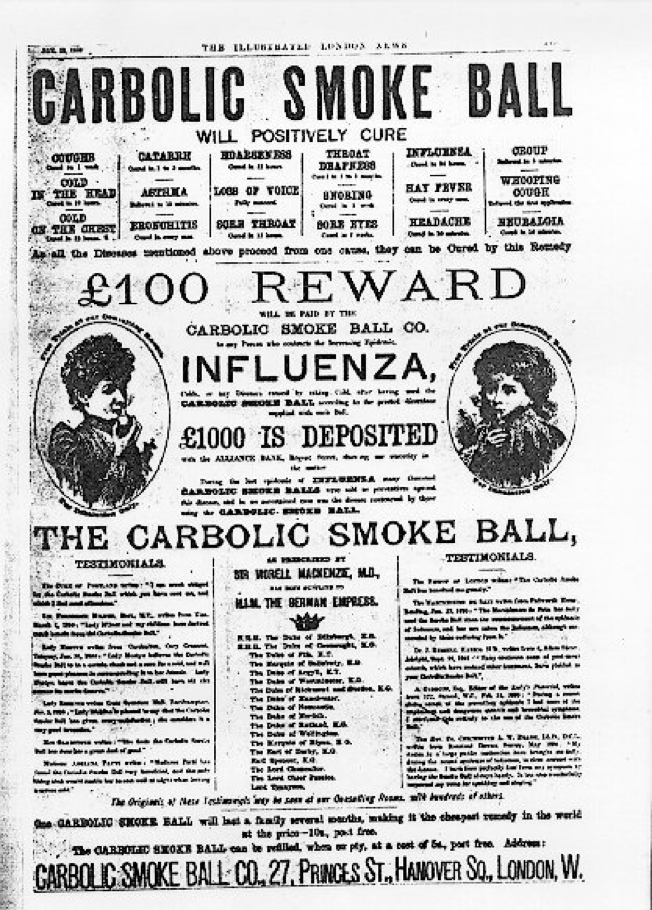
\includegraphics[width=0.5\textwidth]{images/carbolic.png}
\end{center}

\end{frame}



\begin{frame}
\frametitle{Carbolic Ruling}

Lord Justice Lindley discounted that it was a policy, or a bet.

Instead, he said:

\begin{quote}
The first observation I will make is that we are not dealing with any inference of fact. We are dealing with an express promise to pay \textsterling100. in certain events. Read the advertisement how you will, and twist it about as you will, here is a distinct promise expressed in language which is perfectly unmistakable...
\end{quote}

\end{frame}



\begin{frame}
\frametitle{More Recently}

\textit{Bowerman v Association of British Travel Agents, Ltd.}

The tour operator was a member of the association; all members display:

\begin{quote}
	Where holidays or other travel arrangements have not yet commenced at the time of failure [of the tour operator], ABTA arranges for you to be reimbursed the money you have paid in respect of your holiday arrangements. 
\end{quote}

A school's ski trip was cancelled. They were not refunded travel insurance.\\
\quad Should they have been?

\end{frame}



\begin{frame}
\frametitle{More Recently}

Yes, the notice was deemed an offer to contract.

This notice was an offer, and ``created legal relations'' between the school and the travel agency. 

\end{frame}



\begin{frame}
\frametitle{Photocopiers for Sale}

Suppose a salesperson for photocopiers comes to the headquarters of ABC Engineering Inc. 

She offers a sales contract to the receptionist, who signs it, even though his job responsibilities do not include this area.

Is a valid contract formed?

\end{frame}



\begin{frame}
\frametitle{The Answer is Usually ``It Depends...''}

The key question is: does the receptionist have signing authority for the corporation?

A corporation is a ``legal person'' and can enter into a contract.

If, however, the receptionist lacks the signing authority, he cannot bind the corporation to the contract.

If he attempted to do so, the course would find that the corporation did not have intent to enter into the contract; there was no ``meeting of the minds''.

When the receptionist does have this authority, the contract is valid.

\end{frame}



\begin{frame}
\frametitle{Intention to Create Legal Relations}

Parties must have the intention to create legal relations between themselves.\\
\quad That is, they must both want to create a legally-enforceable arrangement.

In dealings of commerce or between strangers, the presumption is strong.

However, this presumption may not hold when a contract is between friends or family members~\cite{lba}.

If Alex invites Terry for dinner, and Terry accepts but does not show, can Alex sue for breach of contract?

\end{frame}



\begin{frame}
\frametitle{Domestic Agreements}

No -- Even if Alex has gone to considerable trouble and expense!

Domestic agreements between husbands and wives, or parents and children, generally do not constitute a legally binding agreement.

\textit{Jones v. Padavatton}, 1968\\
\quad Mother renting a flat out to her daughter.

\textit{Meritt v. Merritt}, 1970 had different circumstances:

They separated and Mr. Merritt signed an agreement to pay the mortgage and then transfer the property to Mrs. Merritt after it was paid off.\\
\quad The separation indicated intent.


\end{frame}



\begin{frame}
\frametitle{Suppliers}

A 2001 case, \textit{Baird Textile Holdings Ltd. v. Marks \& Spencer plc}

The plaintiff had been supplying clothes to M\&S for thirty years when the order was suddenly cancelled.

Baird sued, claiming there should have been reasonable notice because their decades-long dealings implied a contract.

Is Baird correct?

\end{frame}



\begin{frame}
\frametitle{Suppliers}

No - the court held that there was no intent to be legally bound.

Both Baird and M\&S had the option to terminate their arrangement at any time.

If one party wished to be certain that the other would not terminate the agreement on short notice, they could have negotiated a contract to that effect.

One assumes that the other party would wish something in return for that guarantee of notice...

\end{frame}



\begin{frame}
\frametitle{Letters of Intent}
A \alert{letter of intent} is a business document to express interest in proceeding with some action.

A letter of intent that is clearly an ``agreement to agree'' does not constitute a contract.

Letters of intent can establish terms of negotiation, or create moral obligations between the parties.

Can a letter of intent be legally binding?

\end{frame}



\begin{frame}
\frametitle{Letters of Intent}

If it contains all the elements of a contract, yes!

A moral obligation, however, is not legally enforceable.

Consider the case of \textit{Bahamaconsult Ltd. vs Kellogg Salada Canada Ltd.}

The trial judge considered a letter of intent binding, but it was overturned on appeal.

\end{frame}



\begin{frame}
\frametitle{\textit{Bahamaconsult Ltd. vs Kellogg Salada Canada Ltd.}}

The appellate court found:
\begin{quote}
The trial judge found that the document of October 10, 1969, was a contract complete in itself, and that while it was the intention of the parties to draw a further agreement, the subsequent agreement was only to spell out the mechanics of the transfer of the shares, and of the closing of the sale.  With respect, we think that the trial judge erred in so finding.  We are all of the opinion that the document of October 10th does not contain certain essential terms, and that it was the intention of the parties that these terms would be negotiated between them and embodied in a subsequent agreement.  Since the parties were unable to agree upon those terms, there was no enforceable contract.
\end{quote}

\end{frame}



\begin{frame}
\frametitle{Letters of Intent}

Terms set out in a letter of intent are not necessarily going to appear in a contract that follows.

Just because something was agreed upon in the letter of intent, does not mean it has effect, unless it appears in the final contract.

The letter of intent does not affect the contract as interpreted by the courts...\\
\quad(We'll return to this subject soon).

A contract should be carefully reviewed, preferably by a legal expert!


\end{frame}


\part{Contracts: Consideration}

\begin{frame}
\partpage
\end{frame}



\begin{frame}
\frametitle{Consideration}

Black's Law Dictionary:
\begin{quote}
	The cause, motive, price, or impelling influence that induces a contracting party to enter into a contract.
\end{quote}

\alert{Consideration} is something each party promises the other.

Typical example: an engineer designs a product in exchange for a fee.

The engineer has promised a product; the customer has promised money.

\end{frame}



\begin{frame}
\frametitle{Consideration}

Consideration does not have to involve money.\\
\quad A contract can be formed to swap one book for another.

Imagine that you have a friend who is a lawyer. She agrees to draw up your will and power of attorney. 

The service would normally cost \$300, but your friend will do you fa favour. You make a contract in which she agrees to do it for free.

Is this an enforceable contract?

\end{frame}



\begin{frame}
\frametitle{Gratuitous Promise}

No. The lawyer has promised to perform work for you, but you have promised nothing in return.

This is called a \alert{gratuitous promise}. 

Gratuitous promises are not enforceable by law. The law does not prevent them from being fulfilled, but the promisee has no legal remedy if disappointed.

What, if the lawyer agrees to charge you \$1 instead of \$300?

\end{frame}



\begin{frame}
\frametitle{Adequacy of Consideration}

Yes -- now the contract has consideration in the form of \$1.

This seems like a ``bad deal'' for the lawyer, but the courts do not concern themselves with the adequacy of consideration.

As long as there is some consideration, that is enough.

\end{frame}



\begin{frame}
\frametitle{Alternate Consideration}

Recall that a seal, when making an offer irrevocable, is valid as consideration.

The presence of a seal is an outward demonstration that you have, in fact, considered the contract.

Despite the fact you will potentially get nothing out of it!

\end{frame}



\begin{frame}
\frametitle{\textit{Bainbridge v Firmstone}, 1839}

Firmstone requested permission to weigh the two of the boilers.  

Firmstone promised that he would, within a reasonable period of time, return the boilers in good condition.

After weighing the boiler, Firmstone refused to reassemble it claiming that Bainbridge had not received consideration and therefore no legally binding agreement existed.

Was Firmstone correct?

\end{frame}



\begin{frame}
\frametitle{\textit{Bainbridge v Firmstone}, 1839}

Paterson, J. ruled:
\begin{quote}
The consideration is, that Bainbridge, at Firmstone's request consented to allow Firmstone to weigh the boilers.  I suppose Firmstone thought he had some benefit; at any rate, there is a detriment to Bainbridge from his parting with the possession for even so short a time.
\end{quote}

In short: being deprived of something is as much consideration as receiving something.

\end{frame}

\part{Contracts: Capacity}

\begin{frame}
\partpage
\end{frame}



\begin{frame}
\frametitle{Capacity}

For an agreement to be legally binding, each party must be capable of entering into a contract.

That is, they must have the \alert{capacity to contract}.


\end{frame}



\begin{frame}
\frametitle{Age of Majority}

The age of majority is the legally recognized point when one enters adulthood and thus one ceases to be a minor.

At this point, it terminates the legal control and responsibilities of parents or guardians.

It is also the point at which one can enter into a contract.

The age of majority varies by province/territory (18 or 19 depending).

\end{frame}



\begin{frame}
\frametitle{Contracts with Minors}

If a contract is made with a minor, it is not enforceable by the other party.

Exception: the contract concerns providing a necessity of life for the minor, such as food, clothing, shelter...

The minor, however, can enforce the contract on the other party!

The contracting party does not have to know that they are dealing with a minor to be bound to a contract that they cannot have the courts enforce.

Life lesson: check ID.

\end{frame}



\begin{frame}
\frametitle{Reaching Age of Majority}

If a contract is made with a minor, what happens when the minor reaches the age of majority?

The no-longer-minor can disaffirm the contract, otherwise it will be ratified (and binding).

In the case of a minor, lack of capacity is easy to prove; it is established solely by the age of the minor.


\end{frame}



\begin{frame}
\frametitle{Lunatics and Drunkards}

Lunatics and Drunkards~\cite{lba}\footnote{This is really the terminology in a 1970s textbook. How things change!} are also protected by the law.

A ``lunatic'' is mentally incompetent due to illness or disease of some sort. 

A drunk person, or one similarly incapacitated through the use of drugs, is treated in the same way as a minor.

A contract about necessities is binding.

Otherwise it is enforceable only in one direction, as it is for the minor...

\end{frame}



\begin{frame}
\frametitle{``I'm never drinking again...''}

When a drunk or insane person becomes sober or sane again, he or she has a problem of evidence.

He or she must prove that he or she was so intoxicated or insane that he or she did not have the capacity to enter into a contract.

A contract can be ratified upon sobering up (or becoming sane again)...

Repudiation must be prompt upon emerging from the state of incapacity.


If the afflicted party accepts benefits of the contract, it cannot be repudiated.

\end{frame}



\begin{frame}
\frametitle{Corporations}

The objects of a corporation must be stated in the constitutive documents of incorporation.

	Any endeavour that is not allowed for under the objects of incorporation are \textit{ultra vires}, and thus, beyond the power of the corporation.

	Any contract that is \textit{ultra vires} is unenforceable.

This, unfortunately, is an extremely complicated subject and legal advice is highly recommended.

\end{frame}

\part{Contracts: Legality}

\begin{frame}
\partpage
\end{frame}



\begin{frame}
\frametitle{Legality}

A contract that is contrary to a statute will be illegal or void (unenforceable).

Some examples from~\cite{lpe}:
\begin{itemize}
	\item Violates provisions of the Bankruptcy and Insolvency Act.
	\item Contrary to the provisions of the Competition Act.
	\item For services where the party  to perform is required to be licensed.
\end{itemize}

A contract that is incongruent with common-law precedents will also not be enforceable.

\end{frame}



\begin{frame}
\frametitle{Legality}

Common law precedent holds that a contract that is against public policy may be illegal or void.

Public policy doctrine are those principles that form the social, moral and economic foundation of the state.

What is public policy relevant to engineering? Freedom of Trade.

\end{frame}



\begin{frame}
\frametitle{Contrary to Public Policy}

A term in a contract that restricts trade may be seen as contrary to public policy.

Non-competition clauses must continue to allow the individual in question to continue to make a living.

The time and space restraints in non-competition clauses must be reasonable.

Courts will not reinterpret unacceptable non-competition clauses; they will simply render them void.

\end{frame}



\begin{frame}
\frametitle{Obey the Law}

There is also the \alert{doctrine of evasion}.

You cannot enter into a contract simply to evade a responsibility you have to the state.

Example: you cannot enter into a contract for the sole purpose of evading taxes.

Loopholes in the tax code, however, can be exploited.

A contract may not have term to cause a breach of a term in a different contract.

\end{frame}



\begin{frame}
\frametitle{Void versus Illegal}

What is the difference between a void contract and an illegal one~\cite{lba}?

A void contract is simply a failure of the parties to create a binding contract.

If they have partly performed their undertakings, the court will do its best to restore them to their respective positions.

Example: if money was paid or property transferred, the party complaining may be able to show cause to have it returned.

\end{frame}



\begin{frame}
\frametitle{Void versus Illegal}

In a contract that is illegal, the court will refuse to aid a party who knowingly agreed to an illegal purpose~\cite{lba}.

If one party has transferred property to the other, the court will not help him get it back. 

If both parties are involved in the illegal purpose, the court refusing to get involved will technically help the defendant. 

The legal maxim: ``where both parties are equally in the wrong, the position of the defendant is the stronger''~\cite{lba}.


\end{frame}



\begin{frame}
\frametitle{References \& Disclaimer}
\bibliographystyle{alphaurl}
\setbeamertemplate{bibliography item}{\insertbiblabel}
{\scriptsize
\bibliography{290}
}
\vfill

{\tiny Disclaimer: the material presented in these lectures slides is intended for use in the course ECE~290 at the University of Waterloo and should not be relied upon as legal advice. Any reliance on these course slides by any party for any other purpose are the responsibility of such parties.  The author(s) accept(s) no responsibility for damages, if any, suffered by any party as a result of decisions made or actions based on these course slides for any other purpose than that for which it was intended.\par}


\end{frame}


\end{document}

